\chapter{High Energy Physics}
\begin{equation}
    d\sigma \propto |\CM(p_1, p_2 \dots p_n)|^2 \times
    \left(\prod_n \frac{d^3p_n}{(2\pi)^3}\frac{1}{2E_n}\right) \cdot (2\pi)^4\delta^4(p_1 + p_2 - \sum p_n)   
\end{equation}
where
$$ d\prod_n = \left(\prod_n \frac{d^3p_n}{(2\pi)^3}\frac{1}{2E_n}\right) \cdot (2\pi)^4\delta^4(p_1 + p_2 - \sum p_n) $$
is the phase space part.
\begin{itemize}
    \item cross section for collision:
	$$ \sigma = \frac{W_{fi}}{N_i v_i} = \frac{2\pi}{\hbar}|\CM_{fi}|^2 \frac{\rho_f}{N_i v_i} $$
	where$\rho_f = \frac{1}{(2\pi\hbar)^3} p^2_f \frac{dp_f}{dE_0}d\Omega = \frac{1}{(2\pi\hbar)^3} \frac{p_f^2}{v_f}d\Omega $
	$v_i$, $v_f$ are relative velocity of the inital (final) state. $E_0 = \sqrt{s}$
    \item decay width (in GeV) of a particle to a final state f:
	$$ \Gamma_f = \hbar W_{fi} = 2\pi |\CM_{fi}|^2 \rho_f $$
	for 2-body decay of a particle of mass $m_i$ at rest:
	$$ \rho_f = \frac{1}{(4\pi)^2}\frac{p_f}{m_i^2} $$
	$$ \Gamma = \sum_f \Gamma_f \qquad \CB_f = \frac{\Gamma_f}{\Gamma} \qquad \tau = \frac{hbar}{\Gamma} $$
	decay length of a moving particle
	$$ L = \gamma\beta c\tau $$
    \item Massless particles do not have spin as massive particles do. They have 
	helicity
\end{itemize}

%%%%%%%%%%%%%%%%%%%%%%%%%%%%%%%%%%%%%%%%%%%%%%%%%%%%%%%%%%%%%%%%%%%%%%%%
\section{Standard Model}
\tikzstyle{arrow} = [-{stealth[scale=1.5]},rounded corners,thick]
\tikzstyle{split} = [text width = 3cm,text centered]
\begin{figure}[h]
\centering
\begin{tikzpicture}
    \node (CM) [split] {Classical \\ Mechanics};
    \node (QM) [split,right = 1 of CM] {Quantum \\ Mechanics};
    \node (RFT) [split,below = 1 of CM] {Relativistic \\ Field Theory};
    \node (RQFT) [split,below = 1 of QM] {Relativistic \\ Quantum \\ Field Theory};
    \draw [arrow] (QM) -- node [midway,above] {\scriptsize $\hbar \rightarrow 0$}(CM);
    \draw [arrow,transform canvas={xshift=-4pt}] (CM) -- node [midway,left] {\scriptsize $N \rightarrow \infty$}(RFT);
    \draw [arrow,transform canvas={xshift=4pt}] (RFT) -- node [midway,right] {\scriptsize $c \rightarrow \infty$}(CM);
    \draw [arrow,transform canvas={xshift=-4pt}] (QM) -- node [midway,left] {\scriptsize $N \rightarrow \infty$}(RQFT);
    \draw [arrow,transform canvas={xshift=4pt}] (RQFT) -- node [midway,right] {\scriptsize $c \rightarrow \infty$}(QM);
    \draw [arrow] (RQFT) -- node [midway,above] {\scriptsize $\hbar \rightarrow 0$}(RFT);
\end{tikzpicture}
\end{figure}
where N is the number of d.o.f.
\begin{itemize}
    \item The SM doesn't predict the mass or coupling of any particles, it
	relates the masses and couplings to one another.
    \item Looking for high momentm quarks in the nucleon is like looking for
	Mafia in Sicily -- everybody knows they are there, but it's hard to 
	find the evidence!
\end{itemize}

Questions:
\begin{itemize}
    \item How to identify the Lagragian? what requirements should it satisfy?	\\
	A: Guess it, base on the field form and symmetries. start from the 
	simplest terms
    \item How a photon resolve the structure of a proton? Why the smaller the 
	wavelength, the better the resolution?
	A: wave diffraction, the smaller the object (compared to the wavelength),
	the smaller the interference due to scattering.

    \item How to identify generators for a SU(N) group?
    \item What should be physically invariant under transformation?
    \item Yang-Mills theory: how to derive properties from a group of interaction
    \item How do we know the mass of quarks if we can't get free quark
    \item Can neutrino oscillate into anti-neutrino?
\end{itemize}

Do you understand the following terms:
\begin{itemize}
    \item $SU(2)_L \times U(1)_Y$ electroweak theory
    \item Majorana particle
    \item CKM mechanism
    \item BSM mass scale $\Lambda$
    \item The conservation of electric charges is associated with the QED gauge symmetry. 
    \item renormalizable interaction
    \item renormalization scale $\mu$
    \item quantum numbers of the vacuum
    \item Strength of interaction: momentum of the intermedia gauge boson
\end{itemize}
\subsubsection{How to Describe a System}
For any system, firstly determine its possible states and corresponding Hilbert 
space, find out its symmetry group.

%%%%%%%%%%%%%%%%%%%%%%%%%%%%%%%%%%%%%%%%%%%%%%%%
\subsection{QED}
Running coupling constant (from position screening effect due to higher order 
correction)
\begin{equation}
    e_R = e\left[ 1 - \frac{\alpha}{3\pi}ln\left( \frac{\Lambda^2}{m^2}\right) + O(\alpha^2) \right]^{1/2}
\end{equation}
where $\Lambda$ is the cutoff value. Use a measured value to remove cutoff parameter,
\begin{equation}
    \alpha(Q^2) = \frac{\alpha(\mu^2)}{1-\frac{\alpha_0}{3\pi}ln\frac{Q^2}{\mu^2}}
\end{equation}
at low energy $\alpha = 1/137$;
at $M_Z = 90\ GeV$, $\alpha = 1/128$

The gauge invariance of QED is related to the conservation of charge and the
masslessness of the photon.
%%%%%%%%%%%%%%%%%%%%%%%%
\subsubsection{Mesons}
$J^{PC}$
\begin{itemize}
    \item J = L + S
    \item $P = (-1)^{L+1}$
    \item $C = (-1)^{L+:}$
\end{itemize}
For a two-fermion system:
$$ C\ket{f\bar{f}} = (-1)^L (-1)^{S+1}(-1) \ket{f\bar{f}} = (-1)^{L+S}\ket{f\bar{f}} $$

There are two pre-QCD phenomenological frameworks:
\begin{itemize}
    \item Regge phenomenology \cite{PhysRev.108.1063}
    \item Vector Dominance Model (VDM)
\end{itemize}
%%%%%%%%%%%%%%%%%%%%%%%%
\subsubsection{Weak Force and Weak Charge}
Starting from the study of $\beta$ decay, Pauli proposed, reluctantly, the idea
of neutrino to explain the continuum of the energy spectrum of the emitted electron.
Fermi interpretted the decay process as interaction of two currents in analogy to
the EM interaction (Fermi's interaction), the Lorentz invariant amplitude is:
$$ M = G_F (\bar{u}_n ?^\mu u_p) (\bar{u}_{\nu_e}  ?_\mu u_e)$$
the $?$ represents the possible operators. The coupling constant $G_F$ , a parameter
to be experimentally determined, reflects Fermi's original assuption that the 
weak nuclear force has essentially zero range, thus no need for a boson mediator.
It also means massive mediators are needed if the universality of $G_F$ is violated
at high energy scale.

In analogy to EM interaction, the vector nature of the weak current was taken
for granted. But experiments in the 1950s (Wu experiment, 1956) demonstrated 
that parity is not conserved in the weak interaction.
$\beta$ decay of polarized ${}^{60}Co$, angular distribution of decay electrons:
$$ \frac{dN_e}{d\Omega} = 1 - \frac{\vec{\sigma}\cdot\vec{p}}{E} $$
It showes electrons prefer to be emitted opposite to spin direction

Therefore the weak current is not a vector-like
quantity. Among all the bilinear covariants that violate the parity, the one
that "maximally violates" parity is the "V-A" term (what are the other terms???
why this one is choosed???)
$$ M = \frac{G_F}{\sqrt{2}}(\bar{u}_n \gamma^\mu(1-\gamma^5)u_p) (\bar{u}_{\nu_e}\gamma_\mu(1-\gamma^5)\mu_e)$$
The vector-axial term can be rearrange to make it a vector term:
$$ \left( \frac{1-\gamma^5}{2} \right)^2 = \frac{1}{4} (1 - 2\gamma^5 + (\gamma^5)^2) = \frac{1-\gamma^5}{2} $$
$$ \gamma^\mu \frac{1-\gamma^5}{2} = \frac{1+\gamma^5}{2}\gamma^\mu $$
$$ \gamma^\mu \frac{1-\gamma^5}{2} = \frac{1+\gamma^5}{2}\gamma^\mu \frac{1-\gamma^5}{2} $$
So the current can be write as:
$$ j^{\mu}_{(p \rightarrow n)} = \bar{u}_n \gamma^\mu \frac{1-\gamma^5}{2} u_p 
    = \bar{u}_n \frac{1+\gamma^5}{2}\gamma^\mu \frac{1-\gamma^5}{2} u_p 
    = \bar{u}_{n, L}\gamma^\mu u_{p, L}$$
$$ j_\mu^{(e \rightarrow \nu_e)} = \bar{u}_{\nu_e, L} \gamma_\mu u_{e, L} $$
$$ M = \frac{4G_F}{\sqrt{2}} j_{(p \rightarrow n)}^\mu j_\mu^{e \rightarrow \nu_e}$$
The current is a vector now, but of only the left-handed spinor. This allow one
to treat weak interaction as a vector theroy, like EM interaction (so that we
can unify them). The cost is the introduction of the notino of a chiral spinor.

Later, physicists introduced massive $W^{\pm}$ to explain the non-universality 
of $G_F$. (??? How ???) But the theory was far from complete, calculations of
anything other than lowest-order, low-energy diagrams lead to very serious
problems. These problems signaled the need for a more complete theory of weak
interactions, one that is on par with QED (a renormalizable theory)

Though of the similar current structure, one thing needs to be noticed is that
the particles change identies at the vertex -- clearly, something novel occurs 
at a weak vertex. The most analogous process in QED is pair annihilation -- 
conservation of charge at the vertex generates the U(1) (global) gauge symmetry.
Looking at the weak interaction again, $n \rightarrow p + e^- + \bar{\nu}_e$, 
$\mu \rightarrow e + \bar{\nu}_e + \nu_\mu$ and $\pi^- \rightarrow l + \bar{\nu}_l$.
Lepton number and charge are conserved in weak interaction, this suggests natural
doublets: $\begin{pmatrix} \nu_l \\ l \end{pmatrix}$. Considering the following 
weak current:
$$ j_\mu^- = \bar{\nu}_{e,L} \gamma_\mu e_L	\qquad j_\mu^+ = \bar{e}_L \gamma_\mu \nu_{e,L} $$
Defining the left-handed doublet $ c_L = \left.\begin{pmatrix} \nu_e	\\ e \end{pmatrix}\right._L $
The two current can be expressed in a more compact way:
$$ j^\pm_\mu = \bar{c}_L \gamma_\mu t^\pm c_L $$
where,
$$ t^+ = \begin{pmatrix} 0  & 1	\\ 0	& 0 \end{pmatrix}   \qquad 
t^- = \begin{pmatrix} 0  & 0	\\ 1	& 0 \end{pmatrix} $$
This expression clearly suggests an SU(2) symmetry (I can't see it clearly). 
Since the first 2 Pauli matrices combine to form the raising and lowering operators.
One is led to consider the third current using the third Pauli matrix:
$$ j_\mu^3 = \bar{c}_L \gamma_\mu \frac{1}{2}t^3 c_L 
    = \frac{1}{2}(\bar{\nu}_{e,L}\gamma_\mu \nu_{e,L} - \bar{e}_L \gamma_\mu e_L) $$
What does this \textbf{neutral current} represent for? A photon exchange? There
are only left handed electron appears in the current and neutrino doesn't 
participate in the EM interaction. This leaves the impression that SU(2) may
not be the relevant symmetry group for the weak interaction. The 
Glashow-Weinberg-Salam model preserves the SU(2) symmetry by postulating that
$j_\mu^3$ is only a part of a more complete neutral current which includes $j_\mn^{em}$ --
the so called $SU(2) \times U(1)$


\subsubsection{Glashow-Weinberg-Salam (GWS) theory}
The GWS model is derived from the gauge symmetry group $SU(2)_L \times U(1)_Y$.
The SU(2) part is generated by a quantity referred to as "weak isospin" and the
subscript L refers to the fact that only left-handed particles couples to the
gauge bosons of SU(2). The group U(1) is generated by the "weak hypercharge".
The interaction Lagrangian is:
$$ \CL = -i \left( g_w \vec{j}_\mu\cdot \vec{W}^\mu + \frac{g}{2}j_\mu^Y B^\mu \right)$$
3 weak isospin currents: $\vec{j}_\mu = \bar{c}_L g^\mu \vec{t} c_L $ couple to
a weak isotriplet of intermediate vector bosons: $\vec{W}^\mu$ with coupling 
strength $g_w$; and the weak hypercharge current: $j_\mu^Y$ couples with strength
$g'/2$ to an isosinglet intermediate vector boson, $B^\mu$

Using a generic doublet: $c_L = \begin{pmatrix} u_1 \\ u_2 \end{pmatrix}$, where
$u_1$ carries one more unit of charge than $u_2$, let's examine the first 2
terms of the dot product in the Lagrangian:
\begin{equation*}
    \begin{aligned}
	& j^1_\mu W^{1\mu} + j^2_\mu W^{2\mu} = \bar{c}_Lg_\mu t_1 c_L W^{1\mu} + \bar{c}_L g_\mu t_2 c_L W^{2\mu}  \\
       =& \begin{pmatrix} \bar{u}_{1L}	& \bar{u}_{2L} \end{pmatrix} g_\mu \frac{1}{2} \begin{pmatrix}	0 & 1	\\ 1 & 0 \end{pmatrix} \begin{pmatrix} u_{1L} \\ u_{2L} \end{pmatrix} W^{1\mu}
        + \begin{pmatrix} \bar{u}_{1L}	& \bar{u}_{2L} \end{pmatrix} g_\mu \frac{1}{2} \begin{pmatrix}	0 & -i	\\ i & 0 \end{pmatrix} \begin{pmatrix} u_{1L} \\ u_{2L} \end{pmatrix} W^{2\mu}	\\
       =& \frac{1}{2} (\bar{u}_{1L}g\mu u_{2L} + \bar{u}_{2L}g\mu u_{1L}) W^{1\mu}	+ \frac{i}{2} (-\bar{u}_{1L}g\mu u_{2L} + \bar{u}_{2L}g\mu u_{1L}) W^{2\mu}	\\
       =& \frac{1}{2} \bar{u}_{1L}g\mu u_{2L} (W^{1\mu} - iW^{2\mu})  + \frac{1}{2} \bar{u}_{2L}g\mu u_{1L} (W^{2\mu}) + i W^{2\mu}	\\
    \end{aligned}
\end{equation*}
Define $W^\pm = \frac{1}{\sqrt{2}} (W^1 \mp iW^2)$ and $j^{\pm} = j^1 \pm ij^2$,
we get:
$$ j^1_\mu W^{1\mu} + j^2_\mu W^{2\mu} = \frac{1}{\sqrt{2}}(j^+_\mu W^{+\mu} + j^-_\mu W^{-\mu}) $$
So one can derive exactly the charged interaction terms from the first 2 weak 
isospin current.

The weak hypercharge current is defined to be the difference of the EM current 
and the third weak isospin current:
$$ j^Y = 2(j^{em} - j^3) $$
In GWS model, the underlying $SU(2)_L \times U(1)_Y$ gauge symmetry break 
simultaneously, producing 2 neutral vector bosons, which are mixing of $W^3$ B:
\begin{equation*}
    \begin{aligned}
	B_\mu &= A_\mu\cos \theta_w - Z_\mu \sin \theta_w	\\
	W_{3\mu} &= A_\mu\sin \theta_w + Z_\mu \cos \theta_w	\\
    \end{aligned}
\end{equation*}
So we can get:
$$ g_e = g_w\sin\theta_w$$
$$ \frac{G_F}{(\hbar c)^3} = \frac{\sqrt{2}}{8}\frac{g_w}{M_w c^2} $$
where: $g_e = g_w\sin\theta_w$ and $M_w = M_z\cos\theta_w$


In contrast to EM and strong force, the strength of the weak force is different
for particles and anti-particles (Charge-Violation), for a scattering process
and its mirror image (Parity-Violation), and for a scattering process and the 
time reversal of that scattering process (Time-Violation).

Weak mixing angle (Weinberg angle):

the mixing of $W^0$ and $B^0$ vector bosons produce massize $Z^0$ and massless
$\gamma$ 
\begin{equation*}
    \begin{pmatrix}
	\gamma	\\
	Z^0	\\
    \end{pmatrix}
    =
    \begin{pmatrix}
	\cos\theta_W	& \sin\theta_W	\\
	-\sin\theta_W	& \cos\theta_W	\\
    \end{pmatrix}
    \begin{pmatrix}
	B^0 \\
	W^0 \\
    \end{pmatrix}
\end{equation*}

It also gives the relationship between the masses of the W and Z bosons:
\begin{equation*}
    m_Z = \frac{m_W}{\cos\theta_W}
\end{equation*}

The angle can be expressed in terms of $SU(2)_L$ and $U(1)_Y$ couplings:
(weak isospin $g$ and weak hypercharge $g'$)
\begin{equation*}
    \cos\theta_W = \frac{g}{g^2 + g'^2}
\end{equation*}
the electric charge is then expressed as: $e = g\sin\theta_W$
\begin{figure}[h]
    \includegraphics[width=0.48\linewidth]{weak_mixing_angle}
    \includegraphics[width=0.48\linewidth]{weak_charge_screening}
\end{figure}

%%%%%%%%%%%%%%%%%%%%%%%%
\subsubsection{Spontaneous Symmetry Breaking (SSB) -- The Highs Mechanism}
The Higgs potential:
$$ V(\phi) = \mu^2\phi^\dag\phi + \lambda(\phi^\dag\phi)^2 \quad \mu^2 < 0, \lambda > 0 $$
Vacuum Expectation Value (VEV):
$$ \nu = \frac{|\mu|}{\sqrt{\lambda}} = \frac{2M|W}{g} = 246\ GeV$$
This is defined as the \textbf{EW scale}

In the SM, the Higgs field is a weak isospin doublet:
\begin{equation}
    \phi = 
	\begin{pmatrix}
	    \phi^+  \\
	    \phi^0  \\
	\end{pmatrix}
      = \frac{1}{\sqrt{2}}
	\begin{pmatrix}
	    \phi_1 + i\phi_2	\\
	    \phi_3 + i\phi_4	\\
	\end{pmatrix}
\end{equation}
A fluctuation around the minimum $\nu$ spontaneously breaks the rotational 
symmetry of the Higgs field.

Choose direction of fluctuation so that:
$$ \phi_0 = \frac{1}{\sqrt{2}} \begin{pmatrix} 0	\\ \nu \\ \end{pmatrix} $$

Then the fluctuation around the minimum $\nu$ will be:
$$ \phi(x) = \phi_0 + h(x) = \frac{1}{\sqrt{2}} \begin{pmatrix} 0	\\ \nu+h(x) \\ \end{pmatrix} $$

The scalar field $h(x)$ describes a physical Higgs boson.
Expanding the Higgs potential to second order in $h^2$:
$$ V = V_0 + \frac{\mu^2}{2}(2\nu h + h^2) + \frac{\lambda}{4} (4\nu^3 h + 6\nu^2 h^2) = V_0 + \lambda\nu^2 h^2 $$

So the $h^2$ terms gives the Higgs boson's mass:
\begin{equation}
    M_H^2 = 2\lambda\nu^2   \qquad M_H = \sqrt{2}|\mu|
\end{equation}

Vector Boson Masses:
coupling of the vacuum Higgs field $\phi_0$ to EW bosons: 
$\left( \frac{g}{2}\vec{\tau}\cdot\vec{W} + \frac{g'}{2}B\right) \phi_0 $:
\begin{equation*}
\CL_H = \frac{1}{8} \left| 
    \begin{pmatrix}
	gW^3 + g'B  & g(W^1 - iW^2) \\
	g(W^1 + iW^2)	& -gW^3 + g'B	\\
    \end{pmatrix}
    \begin{pmatrix}
	0   \\
	\nu \\
    \end{pmatrix}
    \right|^2
\end{equation*}
In terms of physical W and Z bosons this gives:
$$ \left( \frac{g\nu}{2} \right)^2 W^+W^- + \frac{\nu^2}{8}Z^0Z^0 \qquad Z^0 = -gW^3 + g'B $$
We identify these as vector boson mass terms:
$$ M_W = \frac{\nu }{2} \qquad M_Z = \frac{\nu\sqrt{g^2 + g'^2}}{2} $$

Higgs couplings to Fermions:
the scalar Higgs field couples fermion states of opposite helicity:
$$ \CL_f = \frac{g_f}{\sqrt{2}} (\bar{f}_L f_R + \bar{f}_Rf_L)\nu + \frac{g_f}{\sqrt{2}} (\bar{f}_L f_R + \bar{f}_R f_L) h$$
The first term is treated as a fermion mass term:
$$ m_f = \frac{g_f\nu}{2} = \frac{\sqrt{2}g_f M_W\sin\theta_W}{e}$$
\begin{itemize}
    \item The vacuum Higgs field $\nu$ generates the fermion masses $m_f$
    \item The second term is the fermion coupling to the Higgs boson h
    \item The coupling constant $g_f$ is proportional to $m_f$
\end{itemize}
%%%%%%%%%%%%%%%%%%%%%%%%
\subsubsection{Mass of Force Particles}
From classical EM, we know that the potential of charge is:
$$ \phi(r) = \frac{1}{4\pi \epsilon_0}{e}{r} $$
which gives to Maxwell Equation (Gauss law):
$$ \nabla \cdot E = -\nabla^2\phi = \frac{\rho}{\epsilon_0} $$

For Yukawa potential: $\phi(r) = -\frac{g_s^2}{4\pi}\frac{e^{-r/a}}{r}$
where a is a range parameter, denoting the range of `strong' force.
For this potential, we can get a similar equation:
$$ \left(\nabla^2 -\frac{1}{a^2}\right)\phi = g_s^2 \delta(r)$$
If we take $\phi(r)$ as a Broglie-field $\phi(r, t)$, then somehow (???) we can get:
$$ \left( \nabla^2 - \frac{\partial^2}{c^2\partial t^2} - \frac{1}{a^2}\right) \phi(r, t) = 0 $$
the solution to the above equation is:
$$ \phi \propto exp(i(p\cdot r - Et)/\hbar)$$
so we get:
$$ \frac{E^2}{c^2\hbar^2} = \frac{p^2}{\hbar^2} + \frac{1}{a^2}$$
compare to Einstain's energy-momentum relation:
$$ E^2 = (pc)^2 + (m_0c^2)^2$$
we know the mass of the force particle will be:
$$ m_0 = \frac{\hbar}{ac} $$
take the typical strong force range: $a \approx 2 \ fm$, we get $m_0 \approx 100\ MeV$
which is close to the mass of pions, the force particle for transfering strong
interaction.

%%%%%%%%%%%%%%%%%%%%%%%%
\subsubsection{Decay}
I will classify natural process into 3 classes:
\begin{itemize}
    \item Passive: a change caused by outer force
    \item Oscillation: a peirodic movement
    \item Decay: an automatic reversable process
\end{itemize}
Decay is a tricky process, it is reversable but the reversation almost never
happen natually, just like the expansion of theoretical gas from a small box
into a larger space: it is possible that at some time later, the gas will 
gather within the small box again, but that possibility is teeny tiny that 
we can ignore it. So the question is: what's the intrinsic force for decay?
why a particle decay?

\subsubsection{Hard scattering}
In High Energy Physics, people are usually interested only in hard processes,
hard means large momentum transfer -- either a violent scattering (DIS) or creation
of a system of large mass (Drell-Yan/Z). In the first scenario, the higher 
the momentum of the intermediate particle, the better it can prove the inner 
structure of hadrons (according to the uncertainty principle, the higher the 
momentum, the shorter the distance it will travel; so if the density of partons
is not too high, the intermediat particle will interact with only a single parton). 
In the second scenario, it means the creation of large 
mass particles (tau/charm, bottom, top, W/Z, Higgs and possible new particles).
That's also why we frequently hear high-pT events, high moemntum transfer always
means high pT (during the collision event, the colliding energy must transform
into transverse momentum in order to conserve the total energy). 
By the uncertainty principle, the larger the energy, the shorter the 
interaction time, to avoid (neglect) the interference from long-distance strong force 
that holds partons together in the hadron. Theoretically, we can calculate only 
the perturbative processes, which is equivalent to large momentum transfer in 
the scattering process. Following this requirement, pT is a natural candidate 
for trigger. Because pT is invariant under Lorentz transformation, high pT means
large momentum transfer. It is possible to have hard scattering with low pT, 
but they are hard to be distinguished from the large collision backgrounds.
Another reason is that, with high momentum, the intermedia particles can live (travel)
longer due to time dilation effect, which helps to distinguish them. For example,
in DIS, the larger the COM energy s, the shorter the length of hadron in the
collision direction, therefore the shorter the time that electron traverse the
hadron, but the larger the lifetime of virtual partons. If the former (electron
traverse) is much shortre than the latter, then we can safely assume the hadron
is a collection of `free' partons without interactions between them, and each
parton carries a definite fraction x of the hadron's momentum.

The question is how to identify what trigger the hard scattering, or is it 
just a random event with low probability?

\subsubsection{Inclusive, semi-inclusive and exclusive}
From the experimental point of view (final state):

Exclusive means you know every detail (energy, momentum, charge etc.) of every 
final state particle, therefore can exclusively identify one and only one 
well defined physical process (exclude the possibility of other process).

On the other hand, inclusive means we know only those particles that we are
interested in, leaving the other product unmeasured (but we don't care). 
Therefore, include the effect of several specific channels (processes).
for example: e + p -> e' + X; here X means unspecified staff that we don't care about,
so this is an inclusive process.

The most tricky part is semi-inclusive, by its name, semi-inclusive is also
inclusive, but not completely inclusive; we will know a part of the unspecified
staff. for example: ep -> e' + h + X; here we focus on the distribution of a
specific hadron h and sum over all other hadrons that accompany it.



From the theoretical point of view (initial state):

It is hardest to calculate the exclusive process, we need to know the detailed
inner structure of hadrons (PDF, FF) and how partons evolve into hadrons

While inclusive will be much easier, we can simplily treat hadrons as without
inner structure and take the average effect

Finally, semi-inclusive will care about the distribution of one specific parton
inside the hadron, but not all partons.


To sum up, we can analog them to black box detecting:
\begin{itemize}
    \item exclusive means you find out all inner structure of the black box
    \item semi-inclusive means you know part of the inner structure
    \item inclusive means we don't care about the inner structure, we just want
	to know how it react to specific particles
\end{itemize}

%%%%%%%%%%%%%%%%%%%%%%%%
\subsubsection{Diffractive Process}
Diffractive processes are those where the interacting hadrons remain intact or 
dissociate into low mass hadronic systems via an exchange which has vacuum 
quantum numbers, often referred to as a pomeron (P).
In ep collision: $ep \rightarrow eXY$, the final state systems X and Y are 
separated in rapidity. In pp (pA, AA) collisions, one or both hadrons survive 
intact though the strong interaction between them.

Diffractive processes were experimentally first observed by experiments at HERA
collider and experiment UA8 at CERN. Experimentally, diffractive events may be 
selected either by the presence of a large rapidity gap (LRG) in the rapidity 
distribution of the outgoing hadrons or by detecting a leading proton in the 
final state.

\subsubsection{flow of color between jets}

%%%%%%%%%%%%%%%%%%%%%%%%
\subsubsection{Infrared Safety}
The 

%%%%%%%%%%%%%%%%%%%%%%%%
\subsubsection{$\Lambda_{QCD}$}
the strong coupling constant actually depends on energy:
$$ \frac{1}{g^2(E)} = \frac{1}{g^2(E_0)} + K\cdot \ln(E/E_0) $$
$\Lambda_{QCD}$ is such a value that $g(\Lambda_{QCD}) \sim 1 (\Lambda_{QCD} \sim 150 MeV)$; 
$endLambda_{QCD}$ is such a value that $g(\Lambda_{QCD}) \sim 1 (\Lambda_)$; 
with $E >> \Lambda_{QCD}$, it is weakly coupled (asymptotic freedom);
with $E << \Lambda_{QCD}$, it is strongly conpled (confinement)

QCD potential: $V(r) \sim -\frac{1}{r} + \kappa r$, with $\kappa \sim 1 \frac{GeV}{fm}$


%%%%%%%%%%%%%%%%%%%%%%%%%%%%%%%%%%%%%%%%%%%%%%%%
\subsection{Group}
questions:
\begin{itemize}
    \item (irreducible) representation of group, how do we know if a 
	representation is rereducible?
    \item of SO(3), what's the difference between a 3-D vector representation 
	and a 3-D tensor representation. Well, 3-D vector rep. preserve the
	length while the 3-D tensor rep. preserve the asymmetry; what else?
    \item does each group has generator? the number of independent generators?
    \item Each Lie group is characterized by its lie algebra: the commutation relationship
\end{itemize}

ideas:
\begin{itemize}
    \item the idea is that we want particles to be in an irreducible 
	representation of that group, so that the equations of motion can 
	behave nicely under Lorentz transformations, which should leave the 
	physics invariant in the context of relativistic particle physics.
    \item The irreducible rep. of the Lorentz group are known as the (A, B) rep. 
	where A, B are integers or half-integers
    \item The rep $(\frac{1}{2}, 0)$ and $(0, \frac{1}{2})$ are the Weyl rep. 
	Fields transforming on these rep. have spin $\frac{1}{2}$, known as
	chiral fermions. The ones in the $(\frac{1}{2}, 0)$ rep. are called 
	left-handed Weyl fermions and the other one the right-handed Weyl 
	fermions.

	Chiral fermions must be massless because a LI mass term takes both an
	object from the $(\frac{1}{2}, 0)$ rep. and another from the $(0, \frac{1}{2})$
	rep. \textbf{A standalone chiral fermion does not admit a mass term}.
    \item Fields that transforms under the rep. $(\frac{1}{2}, 0) \oplus (0, \frac{1}{2})$ 
	are Dirac fermions, which can be understood as the composite object 
	formed out of two chiral fermions.
\end{itemize}

definition:
\begin{itemize}
    \item group: a group (G) is a set (finite or infinite) of elements g with 
	a defined binary operation that satisfies 4 fundermental properties: 
	\begin{itemize}
	    \item closure: for any $g_1, g_2 \in G$, $g_1g_2 \in G$
	    \item associativity: for all $g_1, g_2, g_3 \in G$, $(g_1g_2)g_3 = g_1(g_2g_3)$
	    \item identity: there exists an $e \in G$ such that for all $g \in G$, $eg = ge = g$
	    \item inverse: for every $g \in G$ there is a $g^{-1} \in G$ such 
		that $gg^{-1} = g^{-1}g = e$
	\end{itemize}
	Note there is \textbf{no} requirement that $g_1g_2 = g_2g_1$.
	If this equality is satisfied it is an \textit{Abelian group}, otherwise
	it is called a \textit{Non-Abelian group}
    \item group order: if a group is finite, the number of elements is called 
	the group order
    \item group action: an action of apply group (G) elements on a set (X) so that:
	$$G \times X \rightarrow X$$
	it requires:
	\begin{enumerate}
	    \item $\phi(e, x) = x$ where e is the identity element of G 
	    \item $\phi(g, \phi(h, x)) = \phi(gh, x)$ for all $g, h \in G$
	\end{enumerate}
	In this case, G is called a transformation group, X is called a G-set
	and $\phi$ is called the group action
    \item group representation: a representation of a group G is a group action 
	on a vector space V by invertible linear maps.

	Most groups have many different representation
    \item Abelian group: group operation is commutative (all pairs of elements
	commute)
    \item Non-Abelian group: at least one pair of elements doesn't commute
    \item Algebra (Szekeres 2004): ``An algebra consists of a vector space A
	over a field K together with a lwa of composition or product of vectors,
	$\CA \times \CA \rightarrow \CA $ denoted
	$$ (A, B) \rightarrow AB \in \CA \quad (A, B \in \CA)$$
	which satisfies a pair of distributive laws:
	$$ A(aB + bC) = aAB + bAC,  \qquad (aA + bB)C = aAC + bBC $$
	for all scalars $a, b  \in K$ and vectors A, B and C."
    \item Real Lie Algebra: $\CL$ of dimension n ($\ge 1$) is a real vector 
	space of dimension n equipped with a ``Lie product" or commutator [a, b]
	defined for every a and b of $\CL$ such that:
	\begin{enumerate}
	    \item $[a, b] \in \CL$
	    \item $[\alpha a + \beta b, c] = \alpha [a, c] + \beta [b, c]$ for 
		all real number $\alpha, \beta$
	    \item $[a, b] = -[b, a]$
	    \item Jacobi identity holds:
		$[a, [b, c]] + [b, [c, a]] + [c, [a, b]] = 0$
	\end{enumerate}
\end{itemize}

examples:
\begin{itemize}
    \item orthogonal group of degree O(n): the group of $n \times n$ orthogonal 
	matrices, with the group operation of matrix multiplication.
	$$ AA^T = I \Rightarrow A^T = A^{-1}$$
	The orthogonal matrices are the solutions to the $n^2$ equations:
	so only $n(n-1)/2$ elements are independent
    \item SO(n): the determinant of an orthogonal matrix is either 1 or -1,
	$$ det(I) = det(AA^T) = det(A)det(A^T) = det^2(A) \Rightarrow det(A) = \pm 1$$
	so O(n) has tow components (subgroups). The component containing the 
	identity is the special orthogonal group SO(n)
    \item unitary group of degree n U(n): the group of $n \times n$ unitary 
	matrices, with the group operation of matrix multiplication.
	$$ U^\dag U = UU^\dag = I \Rightarrow U^\dag = U^{-1} $$
	for unitary matrices of degree 2, the general expression is:
	\begin{equation*}
	    U = 
	    \begin{pmatrix}
		a   & b	\\
		-e^{i\varphi} b^* & e^{i\varphi}a^* \\
	    \end{pmatrix},
	    \quad
	    |a|^2 + |b|^2 = 1
	\end{equation*}
	It can also be written as:
	\begin{equation*}
	    U =
	    e^{i\varphi/2}
	    \begin{pmatrix}
		e^{i\varphi_1} \cos\theta & e^{i\varphi_2}\sin\theta \\
		-e^{-i\varphi_2} \sin\theta & e^{-i\varphi_1}\cos\theta \\
	    \end{pmatrix}
	\end{equation*}
	take $\varphi_1 = \psi + \Delta$ and $varphi_2 = \phi - \Delta$
	\begin{equation*}
	    U =
	    e^{i\varphi/2}
	    \begin{pmatrix}
		e^{i\psi}   & 0	\\
		0   & e^{-i\psi}    \\
	    \end{pmatrix}
	    \begin{pmatrix}
		\cos\theta  & \sin\theta    \\
		-\sin\theta & \cos\theta    \\
	    \end{pmatrix}
	    \begin{pmatrix}
		e^{i\Delta} & 0	\\
		0   & e^{-i\Delta}  \\
	    \end{pmatrix}
	\end{equation*}
	and another factorization:
	\begin{equation*}
	    U =
	    \begin{pmatrix}
		\cos\alpha  & -\sin\alpha    \\
		\sin\alpha & \cos\alpha    \\
	    \end{pmatrix}
	    \begin{pmatrix}
		e^{i\xi}   & 0	\\
		0   & e^{-i\eta}    \\
	    \end{pmatrix}
	    \begin{pmatrix}
		\cos\beta  & \sin\beta    \\
		-\sin\beta & \cos\beta    \\
	    \end{pmatrix}
	\end{equation*}
    \item SU(n): special unitary group of degree n, same as SO(n), it requires
	$det(U) = 1$. e.x.
	\begin{equation*}
	 SU(2) = \left\{ 
	    \begin{pmatrix}
		\alpha	& -\bar{\beta}	\\
		\beta	& \bar{\alpha}	\\
	    \end{pmatrix}
	    : \quad
	    \alpha, \beta \in C, |\alpha|^2 + |\beta|^2 = 1
	\right\}
	\end{equation*}

	The rank of the SU(N) group is the maximum number of commuting 
	generators (equivalent to the \# of diagonal generators). So
	rank(SU(N)) = N-1.

	M-dim representation of SU(N) ($M\ge N$): element U of the SU(N) group 
	may be represented by $M \times M$ matrices D(U) with $M\ge N$ as long as:
	$$ D(UV) = D(U)D(V) \quad for U, V \in U(N) $$
	D is called an M-dim representation of SU(N).

	If $M=N$, it is the fundamental representation.

	If $M = N^2 -1$, this is called an adjoint representation

	In SM:
	\begin{itemize}
	    \item Matter fields are in the fundamental representation
	    \item Fouce fields are in the adjoint rep.
	\end{itemize}

    \item Lorentz group: is the group L of time-preserving linear isometries 
	of Minkowski space $R^{(3,1)}$ with the Minkowski metric $g= diag(-1, 1, 1, 1)$
	$$ g = \Lambda^T g \Lambda $$
    \item Poincare group: semidirect sum of Lorentz group and translation group
\end{itemize}


\subsubsection{Parton Distribution Function (PDF) and Hadron Fragmentation Function (FF)}
\begin{figure}
    \begin{tikzpicture}[every node/.style = {align = center}]
	\node[ellipse, draw] (n0) {Wigner Distribution \\ $W(x, r, p_T)$};
	\node [ellipse, draw, above right=of n0] (n1) {TMD \\ $f(x, p_T)$};
	\node[ellipse, draw, right=of n1] (n2) {PDF \\ $f(x)$};
	\node [ellipse, draw, below right=of n0] (n3) {GPD \\ $H(x, \xi, t)$};
	\node [ellipse, draw, right=of n3] (n4) {Form Factors \\ GE, GM};
	\draw[-stealth, thick] (n0) -- (n1) node[midway, above, sloped] {$\int d^3x$};
	\draw[-stealth, thick] (n1) -- (n2) node[midway, above, sloped] {$\int d^2p_T$};
	\draw[-stealth, thick] (n0) -- (n3) node[midway, above, sloped] {$\int d^2p_T$};
	\draw[-stealth, thick] (n3) -- (n4) node[midway, above, sloped] {$\int dx$};
    \end{tikzpicture}
\end{figure}

hadron production of $p_T$ and rapidity y from AA collision can be described by:
\begin{equation*}
\frac{d\sigma^{AA\rightarrow h + X}}{dp_T dy} = 
    \int \frac{dx_2}{x_2}\frac{dz}{z} \sum_{i,j}x_1 f_{i/A}(x_1, Q^2)x_2 f_{j/A}(x_2, Q^2)
    \times \frac{d\hat{\sigma}^{ij\rightarrow k}}{d\hat{t}}D_{k\rightarrow h}(z, \mu_F^2)
\end{equation*}
where $\mu_F$ is the renormalization, fragmentation and factorization scales,
taken as $\mu_F = p_T$
\begin{itemize}
    \item PDF: $f(x_B, Q^2)$ where $x_B$ is the Bjorken-x; we expect x to satisfy:
	$ 0 < x < 1$, otherwise some hadrons need to move in opposite direction
	to the hadron, an unlikely configuration.
	\begin{itemize}
	    \item \href{https://lhapdf.hepforge.org/pdfsets.html}{LHAPDF}: 
		collection of PDF sets
	    \item proton PDF: CTEQ
	    \item EPS09 nuclear correction
	\end{itemize}
    \item FF: $D(z_h, Q^2)$ where $z_h$ is the momentum fraction -- the inverse
	of PDF
    \item Modification: of course, this is the simplest form, for real world,
	we need to consider all kinds of modification to this formula, e.x. 
	multi-scattering, initial/final state radiation, which will transfer
	$x_i$ into $\tilde{x}_i = x_i + \Delta x$ and PDF will also be 
	modified correspondingly.
    \item Hadronization models: hadronization can be further divided into 
	fragmentation and decays
	\begin{itemize}
	    \item Independent fragmentation -- not used anymore
	    \item LUND string fragmentation -- PYTHIA/JETSET
		$$ f(z) \propto z^{-1}(1-z)^a \cdot exp\left( \frac{-bm^2_{\perp}}{z} \right) $$
		where z is defined as $z\equiv E/\nu$, E is the hadron energy and
		$\nu$ is the energy transfer; $m^2_\perp \equiv m^2 + p^2_\perp $
		a and b are tunable Lund parameter that determine how to distribute
		available energy to the produced hadrons. Larger a and smaller b 
		shift the FF to a lower z region. Their values are determined
		experimentally, the default value of a and b in PYTHIA6.3 are 
		0.3 and 0.58 $GeV/c^2$ respectively.
	    \item cluster fragmentation -- HERWIG. See \cite{Duncan2019}
		for details of hadronization algorithm.
	\end{itemize}
\end{itemize}

Dokshitzer-Gribov-Lipatov-Altarelli-Parisi (\textbf{DGLAP}) evolution equation 
(evolution of parton density functions: probability for quark to radiate gluon
and for gluon to produce quark-antiquark pairs):
\begin{equation*}
    \frac{d}{d\ln\mu}
    \begin{pmatrix}
	q(x, \mu)   \\
	g(x, \mu)   \\
    \end{pmatrix}
    =
    \int_x^1 \frac{dz}{z}
    \begin{pmatrix}
	\CP_{qq}    & \CP_{qg}	\\
	\CP_{gq}    & \CP_{gg}	\\
    \end{pmatrix}_{(z, \alpha_s)}
    \begin{pmatrix}
	q(x/z, \mu) \\
	g(x/z, \mu) \\
    \end{pmatrix}
\end{equation*}
or
\begin{equation*}
    \mu\frac{\partial}{\partial_\mu}D_i(x, \mu) = 
    \sum_j \int_x^1 \frac{dz}{z}\frac{\alpha_s}{2\pi}P_{ji}(z, \alpha_s) D_j(\frac{x}{z}, \mu)
\end{equation*}

Splitting functions 
\begin{equation*}
    P_{ji}(x, \alpha_s) = P_{ji}^{(0)} + \frac{\alpha_s}{2\pi}P_{ji}^{(1)}
\end{equation*}
at leading order:
\begin{equation*}
    \begin{aligned}
	P^{(0)}_{g \rightarrow qq}(x) &= C_F \frac{1+x^2}{1-x}	\\
	P^{(0)}_{q \rightarrow qg}(x) &= \frac{1}{2} [x^2 + (1-x)^2 ]	\\
	P^{(0)}_{q \rightarrow gq}(x) &= C_F \frac{1+(1-x)^2}{x}	\\
	P^{(0)}_{g \rightarrow gg}(x) &= 2C_A \left[ \frac{x}{1-x} + \frac{1-x}{x} + x(1-x)\right]\\
    \end{aligned}
\end{equation*}
At small x, $P_{qp}$ and $P_{gg}$ dominate.
why $P_{qg}$ is different from $P_{gq}$ ???

\subsubsection{Transverse Momentum Distribution (TMD)}
\begin{itemize}
    \item First global extraction of TMD: Anselmino et al., 2007
\end{itemize}
%%%%%%%%%%%%%%%%%%%%%%%%
\subsubsection{Form Factors (FF)}
\textbf{Note that $F_{1,2}(q^2)$ in elastic scattering is different from
$F_{1,2}(x)$ (PDF) in DIS}.

Idea of FF is similar to diffraction of plane wave in optics. Finite size of 
scattering center introduces a phase difference between plane waves "scattered
from different points in space". If wavelength is long compared to size of the
scattering center, then all scattered waves in phase -- that's why we use
wavelength as the spatial resolution in particle detection.

FF is an interference effect, coherent scattering from charges all over the source.
FF always reduce the corresponding point-source cross-section.
\begin{figure}
    \includegraphics[width=\linewidth]{FF}
\end{figure}

FF encodes information about the charge structure of the nucleon.
$$ \bra{N(P')} J^\mu_{EM}(0) \ket{N(P)} = \bar{u}(P')\left[ \gamma^\mu F_1^N(Q^2) + i\sigma^{\mu\nu}\frac{q_v}{2M}F_2^N(Q^2) \right] u(P) $$ 
Sachs FF: $G_E = F_1 - \tau F_2$; $G_M = F_1 + F_2$; $\tau = \frac{Q^2}{4M^2}$
where
\begin{itemize}
    \item $F_1$: non-spin flip (Dirac FF) describe the charge distribution
    \item $F_2$: spin flip (Pauli FF) describe the magnetic momentum distribution
\end{itemize}

When $q^2 = 0$
\begin{itemize}
    \item $G_E = 1$
    \item $G_M = \mu$
    \item $\mu \frac{G_E^p}{G_M^p} = 1$
\end{itemize}

When $q^2$ is small
\begin{itemize}
    \item $G_E(q^2) \approx G_E(\vec{q}^2) = \int e^{i\vec{q}\vec{r}} \rho(\vec{r}) d^3\vec{r}$
    \item $G_M(q^2) \approx G_M(\vec{q}^2) = \int e^{i\vec{q}\vec{r}} \mu(\vec{r}) d^3\vec{r}$
\end{itemize}

How to measure FF?
\begin{itemize}
    \item Rosenbluth sepeartion method: measure the electron-unpolarized proton 
	elastic scattering xsection at fixed $Q^2$ by varying the scattering angle: $\theta$;
	this method is sensitive to the radiative correction
	$$ \frac{d\sigma}{d\Omega} = \frac{\alpha^2 E' \cos^2(\theta/2)}{4(1+\tau)E^3\sin^4(\theta/2)}
	    \left[ G_E^2 + \frac{\tau}{\epsilon}G_M^2 \right]
	$$
	$$ \frac{d\sigma}{d\Omega}\frac{\epsilon(1+\tau)}{\sigma_{Mott}} = G_E^2\epsilon + \tau G_M^2 $$
	where $\tau = \frac{Q^2}{4M^2}$ and $\epsilon = \left[ 1+2(1+\tau)\tan^2(\theta/2) \right]^{-1}$
    \item Polarization Transfer Technique: measure the recoiled proton's polarization
	from the elastic scattering of polarized electron-unpolarized proton. 
	This method is less sensitive to radiative correction, and insensitive to 
	the absolute polarization, or the analyzing power.
	$$ \frac{G_E}{G_M} = -\frac{P_T}{P_L}\frac{(E+E')\tan(\theta/2)}{2M}$$
	where: $ P_L = M^{-1}(E+E')\sqrt{\tau(1+\tau)}G_M^2\tan^2(\theta/2)$ is the
	polarization along q; $P_T = 2\sqrt{\tau(1+\tau)} G_EG_M\tan(\theta/2)$
	is the polarization perpendicular to q (in the scattering plane)
	and finally $P_N = 0$ is the polarization normal to the scattering plane.
    \item Double-Spin Asymmetry: measure the xsection asymmetry between '+' 
	and '-' electron helicity states in elastic scattering off a polarized 
	proton. 
	$$ A = \frac{-br\sin\theta^*\cos\phi^* - a\cos\theta^*}{r^2 + c}$$
	$$ \frac{G_E}{G_M} = -\frac{b}{2A}\sin\theta^*\cos\phi^* + \sqrt{\frac{b^2}{4A^2}\sin^2\theta^*\cos^2\phi^*-\frac{a}{A}\cos\theta^* - c}$$
	where: $r = G_E/G_M$, a, b, c are kinematic factors, $\theta^*$ and $\phi^*$ are pol.
	and azi. angles between $\vec{q}$ and $\vec{S}$
    \item There is dramatic discrepency between Rosenbluth and recoil polarization
	technique, the possible explanation is the Two Photon Exchange (TPE) \cite{PhysRevC.76.035205}
\end{itemize}

%%%%%%%%%%%%%%%%%%%%%%%%
\subsubsection{Symmetry}
When we say that nature is invariant under some symmetry, it means
\begin{itemize}
    \item  All objects in the theory have well defined transformation properties 
	(i.e., well defined ``representation" of the symmetry group) under the symmetry,
    \item Every interaction is invariant (i.e., a ``singlet") under the symmetry transformations
\end{itemize}
The ``objects" of particle physics are particle fields.
The interactions in particle physics are the operators in the lagrangian.

\subsubsection{C, P and T symmetry}
This was first observed in charged current (exchange of W+ or W- particles) 
interactions in 1956, by Madame Wu and collaborators studying the radioactive 
decay of 60Co (isotope 60 of Cobalt). Parity violation in neutral current 
(exchange of Z0 particles) scattering interactions was first observed at SLAC 
in 1978, by Charles Prescott and collaborators studying the scattering of 
electrons from protons in a liquid deuterium target.

Parity is maximally violated in weak interaction, so is C-parity.

Symmetry conservation and non-conservation (violation) can have dramatic effects 
for both particle physics and cosmology. The combined symmetry CPT is believed 
to be conserved for all particle interactions. Consequences of CPT symmetry are 
that a particle and its anti-particle should have the same mass and lifetime.
No violations of CPT have yet been observed. CP violation, however, has been 
observed as discussed below. CP violation is especially intriguing, since it 
is believed to be a necessary ingredient to explain the preponderance of matter 
over antimatter in the universe -- ie. to explain why we exist at all!

Charge (C) Violation is also observed in weak interactions, but not in 
electromagnetic or strong interactions. C Violation occurs when the rate for a 
particle interaction is different if all the particles in the interaction are 
changed to anti-particles. C Violation was first demonstrated in 1957 by 
physicists at the University of Liverpool studying the decay of muons to 
electrons and anti-muons to positrons and then analyzing the polarization of 
the electrons and positrons.  It was found that muons decayed to left-handed 
electrons but not to right-handed electrons, and that anti-muons decayed to 
right-handed positrons but not to left-handed positrons.

When C and P Violation were first observed in 1956 and 1957, it was expected 
that when C and P operations were combined together (the CP operation), 
symmetry would still be preserved.  Otherwise, CP violation would necessarily 
imply T violation in order to conserve CPT. However, CP was observed to be 
violated at a small level in the weak interactions of kaons (particles that 
contain a down-type quark and a strange-type quark) in 1964 by James Cronin 
and Val Fitch and collaborators, for which they won the Nobel Prize in physics 
in 1980. Recently, CP violation has also been observed in the weak interactions 
of particles involving bottom quarks. This is the main program for the BaBar 
experiment at SLAC.

Time (T) Violation has also been observed in the weak interactions of kaons by 
the CPLEAR experiment at CERN and the KTEV experiment at Fermilab. T Violation 
means that the rate for a particle interaction is different for the time-reversed process.

CPT theorem:
\textbf{All interactions described by a local Lorentz invariant gauge theory
must be invariant under CPT}

test of CPT invariance:
\begin{itemize}
    \item Particles and antiparticles have equal masses:
	$$ M(K^0) - M(\bar{K}^0) < 10^{-19} (M(K^0) + M(\bar{K}^0)) $$
    \item Particles and antiparticles have equal lifetime:
	$$ \tau(\mu^+) - \tau(\mu^-) < 10^{-4} (\tau(\mu^+) + \tau(\mu^-)) $$
    \item Particles and antiparticles have equal and opposite charge:
	$$ Q(p) - Q(\bar{p}) < 10^{-5} e $$
    \item Particles and antiparticles have equal magnetic moments:
	$$ \mu(e^+) - \mu(e^-) < 10^{-12} (\mu(e^+) + \mu(e^-)) $$
\end{itemize}
%%%%%%%%%%%%%%%%%%%%%%%%
\subsubsection{Parity}
$$ P\psi(\vec{r}) = \psi(-\vec{r}) $$
Parity of $\psi$ can be either odd (P = -1) or even (P = +1):
$\psi(x) = \sin kx $ is odd and $\psi(x) = \cos kx$ is even.

Angular part of atomic wavefunctions (associated Legendre pol.):
$$ Y_l^m = P_l^m(\cos\theta) e^{im\phi} $$
$$ PY_l^m = P_l^m(\cos(\theta + \pi)) e^{im(\phi + \pi)} = (-1)^{l+m} \times (-1)^m \times Y_l^m = (-1)^l \times Y_l^m $$

Intrinsic Parity (fermions):
By applying a spatial inversion to the Dirac equation:
$$ \left( i\gamma^0\partial_t -i\vec{\gamma}\vec{\nabla} - m\right)\psi(-\vec{r}, t) = 0 $$
So the parity operator is identified as $P = \gamma^0$
$$ \psi(\vec{r}, t) =  \gamma^0\psi(-\vec{r}, t) = \begin{pmatrix} \CI & 0\\ 0 & \CI \\ \end{pmatrix} \psi(-\vec{r}, t) $$
$$ Pu_1 = Pu_2 = +1 \qquad P\nu_1 = P\nu_2 = -1 $$

What about bosons???
%%%%%%%%%%%%%%%%%%%%%%%%
\subsubsection{Charge Conjugation}
\begin{itemize}
    \item C reverses the sign of the charge and magnetic moment: particle $\rightarrow$ antiparticle
    \item Fermions are not eigenstates of C, so can't define intrinsic C-parity of fundamental fermions
    \item Composite states has C-parity: e.x. mesons
	$$ C = (-1)^{L+S} \qquad C(\pi^0) = +1 \qquad C(\rho^0) = -1 $$
\end{itemize}

%%%%%%%%%%%%%%%%%%%%%%%%
\subsubsection{Time Reversal Operator T}
$$ T\psi(\vec{r}, t) = \psi(\vec{r}, -t) $$
Parity of $\psi$ can be either odd (P = -1) or even (P = +1):
$\psi(x) = \sin kx $ is odd and $\psi(x) = \cos kx$ is even.

\begin{table}
    \begin{tabular}{| l | c | c   c   c |}
	\hline
	Quantity    & Notation	& P & C	& T \\
	\hline
	Position    & $\vec{r}$	& -1	& +1	& +1	\\
	Momentum (Vector)    & $\vec{p}$	& -1	& +1	& -1	\\
	Spin (Axial Vector)    & $\vec{sigma} = \vec{r} \times \vec{p}$	& +1	& +1	& -1	\\
	Helicity    & $\vec{sigma} \cdot \vec{p}$	& -1	& +1	& +1	\\
	Electric Field    & $\vec{E}$	& -1	& -1	& +1	\\
	Magnetic Field    & $\vec{B}$	& +1	& -1	& -1	\\
	Electric Dipole Moment  & $\vec{\sigma} \cdot \vec{E}$	& -1	& -1	& -1	\\
	Magnetic Dipole Moment	& $\vec{\sigma} \cdot \vec{B}$	& +1	& -1	& +1	\\
	Transverse Polarization	& $\vec{\sigma}\cdot(\vec{p}_1 \times \vec{p}_2)$   & +1    & +1    & -1    \\
	\hline
    \end{tabular}
\end{table}
%%%%%%%%%%%%%%%%%%%%%%%%%%%%%%%%%%%%%%%%%%%%%%%%
\subsection{Gauge Theory}
Gauge theory is any field theory in physics in which some global, continuous 
symmetry of the theory is \textbf{promoted} to a local symmetry. By doing so, 
a new field is introduced (the gauge field) which has its own dynamics and 
couples to the particles/fields which have the symmetry. Those particles are 
then said to be charged under the gauge field.

So gauge symmetry is a local symmetry. Note that gauge symmetry is not real 
physical symmetry, it come from the redundant d.o.f. that we use in a theory 
to describe the physical system. (but what about the gauge field, they correspond
to real physical particles; where do they come from?)

e.g. for complex scalar field:
$$ \CL = (\partial_\mu\phi^*)(\partial^\mu\phi) - V(|\phi|) \quad S = \int d^4x\CL $$
This action S has a global, continuous symmetry -- an overall phase:
$$ \phi \rightarrow e^{i\alpha}\phi $$
under this transformation, the action doesn't change. This type of change is
called a gauge transformation, the corresponding symmetry group is the Lie 
group U(1).

Now comes the magic, if we wish not only the global phase symmetry, but also
the local phase symmetry (???why???). Then $\alpha$ will depend on x: $\alpha(x)$.
$$ \phi \rightarrow e^{i\alpha(x)}\phi $$
Obviously, under this local gauge transformation, S is not invariant, it picks
up a new term: $\partial \alpha(x)$ (take the first order of $\alpha$). 
\begin{equation*}
    \begin{aligned}
	\partial_\mu \phi^*\partial^\mu\phi &\rightarrow 
	\partial_\mu (e^{-i\alpha(x)}\phi^*) \cdot \partial^\mu(e^{i\alpha(x)}\phi)	\\
	&= e^{-i\alpha}(\partial_\mu\phi^* - i\phi^*\partial_\mu\alpha) \cdot
	   e^{i\alpha}(\partial^\mu\phi + i\phi\partial^\mu\alpha)  \\
	&= \partial_\mu\phi^*\partial^\mu\phi + 
	    i\partial_\mu\alpha(\phi\partial^\mu\phi^* - \phi^*\partial^\mu\phi) 
	    + \phi\phi^*\partial_\mu\alpha\partial^\mu\alpha \\
	&\approx \partial_\mu\phi^*\partial^\mu\phi + 
	    i\partial_\mu\alpha j^\mu	\\
    \end{aligned}
\end{equation*}
where $j^\mu = i(\phi\partial^\mu\phi^* - \phi^*\partial^\mu\phi)$ is the current,
which satisfies: $\partial_\mu j^\mu = 0$ (the continuity equation). 
So charge is defined as:
$$ Q = \int d^3x j^0 = i\int d^3x (\phi\dot{\phi}^* - \phi^*\dot{\phi}) $$
(charge conjugation: if we transfrom $\phi\rightarrow \phi^*$, then we get
$Q \rightarrow -Q$, that's why this transformation is named as charge conjugation).

To enforce such a symmetry, we need a new
type of derivative $D_\mu\phi$, which transforms in the same fashion as $\phi$:
$$ D_\mu\phi \rightarrow e^{i\alpha(x)}D_\mu\phi $$
This kind of derivative is said to be a gauge covariant derivative, in that it 
transforms in the same fashion as the field under a gauge transformation. To 
construct such a derivation, we need to introduced a new field called the 
\textbf{gauge field} (and its transformation will be prescribed to satisfy the 
gauge covariance). So the gauge covariant derivative is:
$$ D_\mu\phi = \partial_\mu\phi + igA_\mu\phi $$
A is the gauge field. It is playing the role of a connection field. In order to
make the derivative gague covariant, the gauge field transforms as:
$$ A_\mu \rightarrow A_\mu - \frac{1}{g}\partial_\mu\alpha(x) $$
Seeing that $A_\mu$ is required to have derivatives of the group, so the 
connection field is a vector with components which have values in the Lie 
algebra associated with the symmetry group.

So the new action is:
$$ S = \int d^4x(D_\mu\phi^*)(D_\mu\phi) - V(|\phi|) $$
It keeps invariant under the gauge transformation (both local and global).
However, the gauge field is playing a passive role here -- it has no dynamics.
Having introduced a new field, it should play a role in physics. So will add
a kinematic term for it. A kinematic term must have derivatives, but not all
derivative terms are possible -- only those that keeps invariant under gauge
transformation. For U(1), the simplestic kinematic term is: $F_{\mu\nu}F^{\mu\nu}$
where $F_{\mu\nu} = \partial_\mu A_\nu - \partial_\nu A_\mu$
So the final action for the complex scalar theory is:
$$ S = \int d^4x \left[(D_\mu\phi^*)(D^\mu\phi) - V(|\phi|) - \frac{1}{4}F_{\mu\nu}F^{\mu\nu}\right] $$

Another way of introducing Scalar ED from interaction aspect, see 
materials//Complex\_Scalar\_SED.pdf
%%%%%%%%%%%%%%%%%%%%%%%%
\subsubsection{Isospin}
Isospin is a continuous symmetry (additive quantum number) which reflects the 
fact that strong interaction is not sensitive to exchange of proton and neutron.
Because they have similar mass, so we regard them as isospin doublet with 
isospin 1/2, and the quantum state can be written as: ($\frac{1}{2}, \pm\frac{1}{2}$)
In quark model, we know that the isospin comes from u quark and d quark whose 
isospin are defined as ($\frac{1}{2}, +\frac{1}{2}$) and 
($\frac{1}{2}, -\frac{1}{2}$) respectively. Note that only u and d quarks have 
isospin, other 2 generations of quarks: c, s, t, b don't have isospin. 

The isospin of compound particles: though we know the isospin of basic quarks,
there is no theoretical way to calculate the isospin of compound particles if
the component particles have non-zero isospin. But given the component, we can
experimently identify their isospin. for example (according to Clebsch-Gordan Coefficient Table)
$$ \ket{\frac{1}{2}, +\frac{1}{2}}\ket{\frac{1}{2}, -\frac{1}{2}} = 
    \frac{1}{\sqrt{2}}(\ket{1, 0} + \ket{0, 0})$$
so we know that there will be 2 bound state, one with isospin 1 (triplet), the 
other one isospin 0 (singlet), by measuring their mass, we can identify 
$\ket{1, 0}$ because its mass will be similar to 2 other states: $\ket{1, \pm1}$.
For example: $\pi^\pm, \pi^0$ ($\rho^\pm, \rho^0$) forms the triplet therefore 
$\pi^0$ ($\rho^0$) has isospin 1. The left isospin 0 particle is $\eta$ 
($\omega$) -- the lighter singlet and $eta'$ ($\phi$)-- the heavier singlet. 

The problem is why particles in the multiplet should have similar mass, what
about spin multiplet?
     
\subsubsection{Jet Quenching}
Jet will be produced when partons hadronized in vacuum. If the hadronization
happens in a medium rather than the vacuum (e.x. hot QGP or cold nuclear matter),
then the effect caused by the medium is called jet quenching. Specifically,
2 main effects:
\begin{itemize}
    \item change momentum direction (transverse momentum broadering) through
	multiple scattering
    \item parton energy loss due to radiations (dominates at high momentum) and 
	scattering (or bremsstrahlung: dominate at low momentum); in rarely cases,
	parton energy will increase due to scattering
	\begin{itemize}
	    \item BDMPS approach (Radiation energy loss $\Delta E$ in a static
		medium of length L for $E \rightarrow \infty$):
		\begin{equation*}
		    \Delta E \propto \alpha_s C_F \hat{q} L^2 
		    \quad
		    C_F = \left\{ 
		    \begin{aligned}
			3	\quad& \text{for gluon jet}	\\
			4/3	\quad& \text{for quark jet}	\\
		    \end{aligned}
		    \right.
		\end{equation*}
		where medium parameter: $\hat{q} = \frac{\mu^2}{\lambda}$
		$\mu^2$ is the typical momentum transfer from the medium to the parton
		and $\lambda$ is the mean free path
	\end{itemize}
\end{itemize}
For hot QGP, the proton propagate as much as $5-10\ fm$ within the medium.



\subsubsection{Running Strength of Interaction}
3 (EM, weak, strong) of the 4 basic forces display running trait. Running 
means the effective charge varies with energy scale (or distance).
therefore the force strength varies with distance. Actually, we may understand
it the other way, the charge keeps unchanged, but the coupling constant is 
running with the distance. 

For EM and weak interaction, the larger the distance, the smaller the coupling
constant. At long distrance (approximately the width of a proton), the weak charge 
looks smaller because of quantum fluctuations in the vacuum -- every particle is 
surrounded by an ephemeral cloud of particles that effectively form a screen 
between interacting particles.

But strong force acts the opposite way, the larger the distance, the stronger 
the coupling, which is called asymptotic freedom.

%%%%%%%%%%%%%%%%%%%%%%%%%%%%%%%%%%%%%%%%%%%%%%%%
\subsection{Deep Inelastic Scattering (DIS)}
\begin{itemize}
    \item Deep: virtual photon can probe very small distance ($Q^2 >> M^2_p$)
    \item Inelastic: virtual photon destruct the target hadron ($W^2 >> M_p^2$)
\end{itemize}

\begin{figure}[h]
    \centering
    \begin{tikzpicture}
	\tikzset{
	    fermion/.style={very thick, postaction={decorate}, 
		decoration={markings, mark=at position 0.5 with {\arrow{stealth}}}},
	    photon/.style={decorate, decoration={snake}}
	}
	\coordinate (ein) at (-3, 0);
	\coordinate (eout) at (2.5, 1.5);
	\coordinate (a) at (0, 0);
	\coordinate (b) at (0, -2);
	\coordinate (pin) at (-3, -2);
	\coordinate (pout) at (3, -3);
	\coordinate (xmax) at (3, 0);
	\draw[dashed] (a) -- (xmax);
	\draw[-stealth] (0.5, 0) arc (0:30:0.5) node [right, sloped, Red] {$\theta$};
	\draw[fermion] (ein) -- node [above, sloped] {$(E_e, \vec{k})$}(a);
	\draw[fermion] (a) -- node [above, sloped] {$(E_e', \vec{k}')$} (eout);
	\draw[fermion] (pin) -- node [above, sloped] {$(E, 0, 0, -P)$} (b);
	\draw[fermion] (b) -- node [above, sloped] {$(E', P_x', P_y', P_z')$} (pout);
	\draw[photon] (a) -- node [right] {q} (b);
    \end{tikzpicture}
\end{figure}
Ignoring electron's mass: $E_e = k$, $E_e' = k'$ and $E^2 = M^2 + P^2$
\begin{equation*}
    \begin{aligned}
	Q^2 &= -q^2 = (\vec{k} - \vec{k}')^2 - (E-E')^2	\\
	    &= -2kk'\cos\theta + 2EE' \\
	    &= 2EE'(1-\cos\theta) = 4EE'\sin^2\left(\frac{\theta}{2}\right)
    \end{aligned}
\end{equation*}

\begin{equation*}
    \begin{gathered}
	E' = E_e + E - E_e' = \sqrt{M^2 + P_x'^2 + P_y'^2 + P_z'^2} \\
	(E_e + E - E_e')^2 = M^2 + k_x'^2 + k_y'^2 + (k - P - k_z')^2	\\
	EE_e - E_eE_e' - EE_e' = -kP - kk_z' + Pk_z'	\\
	EE_e - E_eE_e' - EE_e' = -E_eP - E_eE_e'\cos\theta + PE_e'\cos\theta	\\
    \end{gathered}
\end{equation*}

%%%%%%%%%%%%%%%%%%%%%%%%
\subsubsection{Low $Q^2$ -- Fixed Target}
$P = 0$, $E = M$
we can get:
$$ M(E_e - E_e') = E_eE_e'(1-\cos\theta) \Rightarrow 
    E_e - E_e' = \frac{2E_eE_e'\sin\left(\frac{\theta}{2}\right)}{M} = \frac{Q^2}{2M}$$
$$ W^2 = (p + q)^2 = M^2 - Q^2 + 2M(E_e - E_e') $$

\begin{itemize}
    \item $Q^2 > 1\ GeV^2$, $W > 2\ GeV$
\end{itemize}

for ep elastic scattering, at high $q^2$ the Rosenbluth expression is:
$$ \frac{d\sigma}{d\Omega} = \frac{\alpha^2}{4E_1^2\sin^4\theta/2}\frac{E_3}{E_1}
    \left( \frac{q^2}{2M^2}G_M^2\sin^2\frac{\theta}{2}\right)$$
The proton magnetic FF is:
$$ G_M(q^2) \approx \frac{1}{(1+q^2/0.71\ GeV^2)^2} \propto q^{-4} \quad high q^2$$
so we get:
$$ \left( \frac{d\sigma}{d\Omega}\right)_{elastic} \propto q^{-6} $$
so the xsection decrease along $q^2$, but this is not what we observe in experiments:
\begin{figure}
    % \includegraphics[width=\linewidth]{ep_inelastic_xsection_over_q2}
    \caption{Phys. Rev. Lett. 23 (1969) 935}
\end{figure}
The plots shows that at high $q^2$, xsection barely depends on $q^2$. Due to
finite size of proton, elastic scattering at large $q^2$ is unlikely, instead
inelastic scattering (where the proton breaks up) dominates.

\includegraphics[width=\linewidth]{DIS_Feynman}
Ignoring partons' transverse momentum and electron's mass:
$$ k = (E_e, \vec{k}) = (E_e, 0, 0, E_e) \quad k' = (E', \vec{k}') = (E'_e, k'_x, k'_y, k'_z) $$
$$ P_h = (E, \vec{P}) = (E, 0, 0, -P)  \quad p = xP_h = (xE, 0, 0, -xP) \quad p' = (E', p'_x, p'_y, p'_z) $$
$$ k^2 = k'^2 = 0 \qquad P_p^2 = P_{p'}^2 = 0 $$
$$ \Downarrow $$
$$ q = (\nu, \vec{q}) = k - k' = (E_e - E'_e, -k'_x, -k'_y, E_e - k'_z) $$
So there are 8 unknown variables in the final state ($E'$ and $E'_e$, $\vec{k}'$ and $\vec{p}'$).
Energy and momentum conservation provide 4 constrains; mass conditions provide 
2 constrains, so there are 2 independent variables in the final state, which are
usually $E'_e$ and $\theta$ (the scattering angle).
$$ E_e + xE = E'_e + E'    \quad p'_x = -k'_x	\quad p'_y = -k'_y  \quad E_e -xE = k'_z + p'_z $$
$$ E'^2 = (E_e + xE - E'_e)^2 = E_e^2 + E'^2_e + (xE)^2 + 2xEE_e - 2E_eE'_e - 2xEE'_e $$
\begin{equation*}
    \begin{aligned}
	E'^2 &= p'^2_x + p'^2_y + p'^2_z = k'^2_x + k'^2_y + (E_e -xE - k'_z)^2	    \\
	     &= k'^2_x + k'^2_y + k'^2_z + E_e^2 + (xE)^2 - 2xEE_e - 2E_ek'_z + 2xEk'_z	\\
	     &= E'^2_e + E_e^2 + (xE)^2 - 2xEE_e - 2E_ek'_z + 2xEk'_z	\\
    \end{aligned}
\end{equation*}
$$ \Downarrow $$
$$ 2xEE_e - E_eE'_e - xEE'_e +E_ek'_z - xEk'_z = 0 $$
$$ \Downarrow $$
$$ k'_z = \frac{E_eE'_e + xEE'_e - 2xEE_e}{E_e-xE} = E'_e\cos\theta $$
$$ q^2 = (E_e - E'_e)^2 - k'^2_x - k'^2_y - (E_e - k'_z)^2 = -2(E_eE'_e - E_ek'_z) = -2E_eE'_E (1 - \cos\theta) $$
$$ x = \frac{E_eE'_e - E_ek'_z}{2EE_e - EE'_e - Ek'_z} = \frac{E_eE'_e - E_ek'_z}{E(E_e - E'_e) - (-E)(E_e - k'_z)} = \frac{Q^2}{2P_h\cdot q} $$

Dynamics (LI variables):
\begin{itemize}
    \item $s = (k + P)^2$
    \item $Q^2 = -q^2 = -(k-k')^2$ 
    \item $y = \frac{P\cdot q}{P\cdot k} = \frac{W^2}{s}$
    \item $x_{Bj} = \frac{Q^2}{2(P\cdot q)} $
    \item $W = (P + q)^2$
\end{itemize}
Important characteristics:
\begin{itemize}
    \item resolution: $Q^2 = -q^2 = 4E_eE'_e\sin^2\left(\frac{\theta}{2}\right)$
    \item energy transfer: $\nu = E - E'$
    \item momentum fraction by a quark: $x = \frac{Q^2}{2P_h\cdot q} = \frac{Q^2}{2M\nu}$
    \item inelasticity: $y = \frac{\nu}{E}$
    \item mass of the hadronic system: $W^2 = (P_h + q)^2 = P_h^2 + 2P_hq + q^2 = $ 
    \item structure functions: $\frac{d\sigma}{dx dQ^2} \propto \alpha^2 Q^{-4}F_2(x, Q^2)$
	\begin{equation*}
	    \begin{aligned}
		F_2(x, Q^2) \rightarrow F_2(x) 
		&= \sum_{q, (\bar{q})} \int_0^1 d\xi e_q^2 \xi q(\xi)\delta(x-\xi) 
		= \sum_{q, \bar{q}} e_q^2 x q(x)    \\
		&= \frac{4}{9}xu(x) + \frac{1}{9}xd(x) + \frac{1}{9}xs(x) + \dots
	    \end{aligned}
	\end{equation*}
	where x is the Bjorken scaling
    \item Parton Distribution Functions (PDFs): u(x), d(x), s(x), etc. are called
	PDFs

	Extraction of PDFs from different beams and targets combinations:
	At any fixed x value:
	\begin{itemize}
	    \item $F_2^{ep} = \frac{4}{9}(u + \bar{u}) + \frac{1}{9}(d + \bar{d}) 
		    + \frac{1}{9}(s + \bar{s}) + \dots$
	    \item $F_2^{en} = \frac{1}{9}(u + \bar{u}) + \frac{4}{9}(d + \bar{d}) 
		    + \frac{1}{9}(s + \bar{s}) + \dots$
		\item $F_2^{\nu p} = 2[d + s + \bar{u} + \dots]$
		\item $F_2^{\nu n} = 2[u + \bar{d} + \bar{s} + \dots]$
		\item $s = \bar{s} = \frac{5}{6}F_2^{\nu N} - 3 F_2^{eN}$
		\item $\sum_q\int_0^1 dx x(q(x) + \bar{q}(x)) = 0.55$ all quarks
		    only carry about half of proton's momentum, the other half
		    is carried by gluons.
	\end{itemize}
	\item How to identify the scattered electrons in ep scattering? What's 
	    its characteristics?
\end{itemize}

SLAC e-p scattering (1969):
\begin{itemize}
    \item electron beam energy: 7-18 GeV
    \item scattering angle: $6-10^\circ$
    \item inclusive approach: only electrons are detected in the final state
\end{itemize}
Unexpected result:
\begin{itemize}
 \item The ratio of $\sigma/\sigma_{Mott}$ has no $Q^2$ dependence and 
     very weak W dependence
 \item Structure function, $\nu W_2$ ($F_2$) has no $Q^2$ dependence
\end{itemize}
Parton model (Bjorken scaling)

\begin{itemize}
    \item First proposed by Richard Feynman
    \item The nulceon is a collection of free, collinear, massless and 
	\textbf{point-like} (therefore no $Q^2$ dependence) partons with 
	spin $1/2$ (??? why 1/2)
    \item Scattering off the nucleon is incoherent sum of elastice scattering 
	off partons.
    \item The probability, f(x) for a parton to carry momentum fraction x,
	does not depend on the process or nucleon energy but is intrinsic 
	property for high energy nucleon
\end{itemize}
Structure function:
\begin{itemize}
    \item Pointlike partons have structure function of the $\delta$ function:
	$$ W_1^i = \frac{Q^2}{4m^2}\delta(\nu - \frac(Q^2){2m})
	 W_2^i = \delta(\nu - \frac{Q^2}{2m})$$
     \item Thr proton sturcture functions are sums over the parton pdfs:
	 $$ W_1 = \frac{F_1(x)}{M}  \qquad F_1(x) = \frac{1}{2}\sum Q_i^2 f_i(x) $$
	 $$ W_2 = \frac{F_2(x)}{\nu}  \qquad F_2(x) = \sum xQ_i^2 f_i(x) $$
	 $$ 2xF_1(x) = F_2(x) $$
     \item Integrate measured FF $F_2$ in electron DIS:
	 $$ \int_0^1 F_2^p(x)dx = \frac{4}{9}f_u + \frac{1}{9}f_d = 0.18 \qquad
	  \int_0^1 F_2^n(x)dx = \frac{4}{9}f_d + \frac{1}{9}f_u = 0.12 $$
	where $f_u = \int_0^1 xu(x)dx = 0.36$ and $f_d = \int_0^1 xd(x)dx = 0.36$ 
	valance quarks are only 54\% of the proton $\Rightarrow$ other partons (gluon)
\end{itemize}

Scaling violation: at high $Q^2$, photon see softer quarks inside quarks (inner
structure due to gluon screening (QCD effect))
$$ F_2(x) \rightarrow F_2(x, Q^2) = x\sum e_q^2(q(x) + \delta q(x, Q^2))$$
where
$$ \delta q(x, Q^2) = \frac{\alpha_2}{2\pi}log Q^2
    \left[ \int_x^1 \frac{dy}{y}q(y)P_{q\rightarrow qg}(x/y) +
    \int_x^1\frac{dy}{y}g(y)P_{g\rightarrow q\bar{q}} -(x/y) \right]$$
%%%%%%%%%%%%%%%%%%%%%%%%
\subsubsection{Polarized DIS}
When target is polarized parallel to beam polarization:
\begin{equation*}
    \Delta\sigma_\parallel = \frac{d^2\sigma}{dE'd\Omega}(\downarrow\Uparrow - \uparrow\Uparrow)
     = \frac{4\alpha^2}{MQ^2}\frac{E'}{\nu E} 
     \left[ (E + E'\cos\theta)g_1(x, Q^2) - \frac{Q^2}{\nu}g_2(x, Q^2) \right]
\end{equation*}
When target is polarized transverse to beam polarization:
\begin{equation*}
    \Delta\sigma_\perp = \frac{d^2\sigma}{dE'd\Omega}(\downarrow\Rightarrow - \uparrow\Rightarrow)
     = \frac{4\alpha^2\sin\theta}{MQ^2}\frac{E'^2}{\nu^2 E} 
     \left[ \nu g_1(x, Q^2) - 2E g_2(x, Q^2) \right]
\end{equation*}

$g_1$ and $g_2$ are analogus to F in unpolarized cross section, they encode 
information about the spin structure of the target nucleon.
\begin{itemize}
    \item $g_1$ is a messure of the spin distribution among the individual 
	constituent quarks (e.g. aligned parallel or anti-parallel to the 
	nucleon spin)
\end{itemize}


%%%%%%%%%%%%%%%%%%%%%%%%%%%%%%%%%%%%%%%%%%%%%%%%
\subsection{$e^+e^-$ Collision}

%%%%%%%%%%%%%%%%%%%%%%%%
\subsubsection{Forward-Backward Asymmetry}
\begin{figure}[h]
    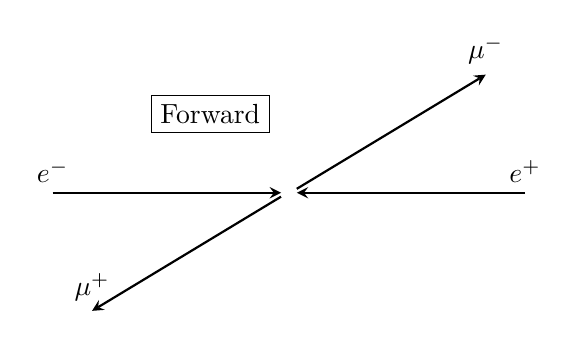
\begin{tikzpicture}
	\draw[thick, -stealth] (-3, 0) node [above, sloped] {$e^-$} -- (-0.1, 0);
	\draw[thick, -stealth] (3, 0) node [above, sloped] {$e^+$} -- (0.1, 0);
	\draw[thick, -stealth] (0.1, 0.05) -- (2.5, 1.5) node [above, sloped] {$\mu^-$} ;
	\draw[thick, -stealth] (-0.1, -0.05) -- (-2.5, -1.5) node [above, sloped] {$\mu^+$} ;
	\node[draw] at (-1, 1) {Forward};
    \end{tikzpicture}
    \qquad
    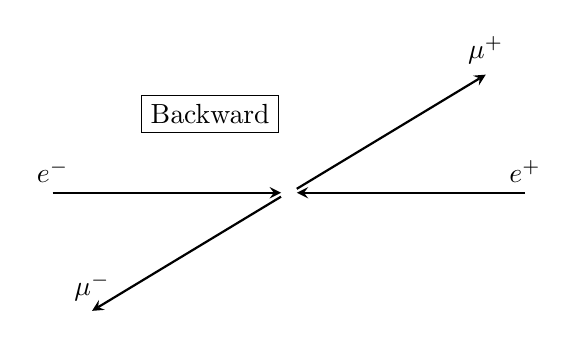
\begin{tikzpicture}
	\draw[thick, -stealth] (-3, 0) node [above, sloped] {$e^-$} -- (-0.1, 0);
	\draw[thick, -stealth] (3, 0) node [above, sloped] {$e^+$} -- (0.1, 0);
	\draw[thick, -stealth] (0.1, 0.05) -- (2.5, 1.5) node [above, sloped] {$\mu^+$} ;
	\draw[thick, -stealth] (-0.1, -0.05) -- (-2.5, -1.5) node [above, sloped] {$\mu^-$} ;
	\node[draw] at (-1, 1) {Backward};
    \end{tikzpicture}
\end{figure}
\begin{equation*}
    A_{FB}^{\mu\mu} = \frac{N_F^{\mu^+} - N_B^{\mu^-}}{N_F^{\mu^+} + N_B^{\mu^-}}
    \approx f(\sin\theta^2\theta_W^{eff}) + \alpha_{QED}(s)\frac{s-m_Z^2}{2s}g(\sin^2\theta_W^{eff})
\end{equation*}

%%%%%%%%%%%%%%%%%%%%%%%%%%%%%%%%%%%%%%%%%%%%%%%%
\subsection{Strong Interaction}
\begin{itemize}
    \item BC Sum Rule\cite{BURKHARDT1970453}: $\int_0^1 g_2(x, Q^2) dx = 0$ 
    \item GDH Sum Rule
    \item Bjorken Sum Rule
\end{itemize}

%%%%%%%%%%%%%%%%%%%%%%%%%%%%%%%%%%%%%%%%%%%%%%%%%%%%%%%%%%%%%%%%%%%%%%%%
\section{Lagrangian}
How does the Lagrandian come:

Consider such a problem that for a given potential and starting/end point, how
to derive its path between the starting and end point. By anology with the 
geometrical optical problem and following the \textbf{Fermat's principle}, it
is natural to argue that there should be a similar principle (quantity): when 
it take minimum (maximum), the path is what nature will choose. 

Now we call that quantity as action S. Obviously, S should be a scalar and it
depends on $q(t)$ -- the possible path. So S is a functional of $q(t)$: $S(q(t))$. 
Consider the physical meaning, $q(t)$'s importance only comes from V(q), so S 
doesn't depend directly on $q(t)$, but on a function of $q(t)$ (we call this 
function Lagrangian):
$$ S = \int \CL(q(t)) $$
So what should $\CL$ integrate over? A natural choice is $dt$ and $d^3x$ because
we know the starting and end points:
$$ S = \int dtd^3x \  \CL(q(t)) $$

Now we come to $\CL$. Obviously, $\CL(q)$ is not enough, because this includes
only potential, but no particle dynamics. For a free particle in vaccum, $\CL(q)$
will be 0. So $\CL$ should only depends on $\dot{q}$:
$$ S = \int dtd^3x \ \CL(q(t), \dot{q}(t)) = \int dtd^3x \ \CL(q, \dot{q}, t) $$
As we said above, $q(t)$ matters just because of $V(q)$, so 
$$ \CL(q, \dot{q}, t) = V(q) + \CL'(\dot{q}) $$
So the position term is energy, then the $\dot{q}$ should also be energy, a 
natural choice is kinematic energy. We can't sum them up, because the total
energy is a constant; so the simplest form for $\CL$ is:
$$ \CL(q, \dot{q}, t) = \lambda \dot{q}^2 - V(q) $$
Here we take the choice of $E_k - E_p$ rather than $E_p - E_k$, the sign doesn't
matter.

One problem is why $\CL$ stops at $\dot{q}$, rather than going on to $\ddot{q} \dots$?
Well, it is insane to think this way. $q$ (potential), $\dot{q}$ (kinematic) is 
state paremeters of a particle, but $\ddot{q}$ is not, it just reflects the 
change of states for a particle.

BTW, for particles, we should add a $\delta(x-p(t))$ to the integral to reflect
the fact that this is a particle rather than a wave. So for particle:
$$ S = \int dt \ L(q, \dot{q}, t) $$
But for fields, the density form should be kept:
$$ S = \int dtd^3x \ \CL(\phi, \dot{\phi}, t) $$

Take extreme (minimum/maximum) value ($\frac{\delta S}{\delta q(t)} = 0$) will
give us the Euler-Lagrange function:
$$ \partial_t\frac{\partial L}{\partial \dot{q}} = \frac{\partial L}{\partial q}$$

%%%%%%%%%%%%%%%%%%%%%%%%%%%%%%%%%%%%%%%%%%%%%%%%
\subsection{QCD}
\begin{itemize}
    \item Asymptotic freedom
    \item Infra-Red Safety (IRS): quantities that are independent of long-distance
	physics. (e.x. once the quark-antiquark pair is produced at short distance,
	the probability for them to turn into some hadron state is unity, 
	independent of the long-distance behavior of the theory). The observable
	must be insensitive to whether n or n+l particles contributed -- as long
	as the n+l particles has n-particles kinematics.
    \item Factorization: physical quantities that can be factorized into long
	distance components (not calculable, but universal) and short-distance
	components (process dependent, but IRS, hence calculable)
\end{itemize}
QCD Lagrangian:
\begin{equation*}
    \begin{aligned}
	\CL_{QCD} &= \bar{q}_i (i\partial_\mu \gamma^\mu \delta_{ij} -
	    g\frac{\lambda^a_{ij}}{2}A_\mu^a\gamma^\mu) - m\delta_{ij}) q_j 
	    - \frac{1}{4}F^a_{\mu\nu}F^{a, \mu\nu}    \\
		&= \bar{q}(i\slashed{D} - m)q - \frac{1}{4}F^a_{\mu\nu}F^{a, \mu\nu}
    \end{aligned}
\end{equation*}
$$ F^a_{\mu\nu} \equiv \delta_\mu A^a_\nu - \delta_\nu A^a_\mu - g f^{abc} A^b_\mu A^c_\nu $$
$$ D_\mu \equiv \partial_\mu + igA^a_\mu \frac{\lambda_a}{2} $$

QCD Beta function
\begin{gather*}
    \frac{d}{d\ln\mu} g(\mu) = \beta{g(\mu)}	\\
    \beta(\mu) = -g\sum_{k=0}\beta_k\left( \frac{\alpha_s}{4\pi}\right)^{k+1} = -\beta_0\frac{g^3}{16\pi^2} - \beta_1\frac{g^5}{(16\pi^2)^2} + \cdots	\\
    \beta_0 = \frac{11N_c - 2n_f}{3}, \beta_1 = \frac{34}{3}N_c^2 - \frac{10}{3}N_cn_f - 2C_F n_f
\end{gather*}

Coupling constant:
\begin{equation*}
    \alpha_s(\mu) = \frac{g^2(\mu)}{4\pi} = \frac{4\pi}{\beta_0\ln\frac{\mu^2}{\Lambda^2_{QCD}}}
    \left[ 1- \frac{\beta_1\ln\ln\frac{\mu^2}{\Lambda^2}}{\beta_0^2\ln\frac{\mu^2}{\Lambda^2}}\right]
\end{equation*}
\begin{itemize}
    \item confinement: $\alpha_s(\mu \rightarrow \Lambda_{QCD}) \rightarrow \infty$
    \item asymptotic freedom: $\alpha_s(\mu \rightarrow \infty) \rightarrow 0$
\end{itemize}

Renormalization group:
\begin{equation*}
    \frac{d\alpha_s(\mu)}{\pi d\ln(\mu^2)} = -\beta(\alpha_s(\mu)) = 
	-\beta_0\left( \frac{\alpha_s(\mu)}{\pi} \right)^2 
	-\beta_1\left( \frac{\alpha_s(\mu)}{\pi} \right)^3 
	+ \cdots
\end{equation*}
\begin{equation*}
    \begin{aligned}
	\alpha_s(\mu) &\approx \alpha_s(M) - \ln\left( \frac{\mu^2}{M^2} \right) \alpha_s^2(M) 
	    + \left( \frac{\beta_0}{\pi} \right)^2 \ln\left( \frac{\mu^2}{M^2} \right) \alpha_s^3(M)    \\
	    &= \frac{\alpha_s(M)}{1+\frac{\beta_0}{\pi}\alpha_s(M)\ln\frac{\mu^2}{M^2}}
	    &= \frac{\pi}{\beta_0\ln\frac{\mu^2}{\Lambda^2}}
    \end{aligned}
\end{equation*}
%%%%%%%%%%%%%%%%%%%%%%%%%%%%%%%%%%%%%%%%%%%%%%%%%%%%%%%%%%%%%%%%%%%%%%%%
\section{Beyond the Standard Model (BSM)}
If there is new physics, are they at larger masses -- energy frontier? Or at
smaller couplings -- intensity frontier? Or both?
\begin{itemize}
    \item Energy frontier -- direct search for new particles, new force and new 
	principles
    \item Intensity frontier -- indirect search through rare processes
    \item Cosmic frontier -- detect high energy particles from cosmic
\end{itemize}

\begin{itemize}
    \item Flavor universality: e.x. the rates of $B^0 (B^+) \rightarrow K^{*0} (K^+) l^+l^-$
	are different for $l=e$ and $l=\mu$; differences are also observed in the
	lepton angular distributions
\end{itemize}
Questions:
\begin{itemize}
    \item Unification: $\alpha_e$, $\alpha_s$ and g can unify (meet) in large energy 
	scale, what will happen if I keep increase the energy?
\end{itemize}
Running coupling constant $\alpha_s$ depends on $Q^2$, a renormalization scale 
$\mu$ is introduced within perturbation theory:
$$ \alpha_s(Q^2) = \frac{\alpha_s(\mu^2)}{1 + (\beta_0\alpha_s(\mu^2)/4\pi)\ln(Q^2/\mu^2)}$$
with $\beta_0 = 11 - \frac{2}{3}n_f$

%%%%%%%%%%%%%%%%%%%%%%%%%%%%%%%%%%%%%%%%%%%%%%%%
\subsection{Grand Unification Theory (GUT)}
\begin{itemize}
    \item Running of $\sin^2\theta_W$
	Loop diagram with $f\bar{f}$ pair couples a $Z^0$ boson to a photon, 
	which are orthogonal states in EW theory:
	$$ \sum Q(I_3 - Q\sin^2\theta_W) = 0 \qquad \sin^2\theta_W = \frac{\sum QI_3}{\sum Q^2} $$
	In a GUT, the sum is taken over a fermion supermultiplet ($\nu_e, e, d_r, d_g, d_b$),
	which gives $\sin^2\theta_W = 0.375$; But at EW scale: $\sin^2\theta_W = 0.22$
\end{itemize}
%%%%%%%%%%%%%%%%%%%%%%%%%%%%%%%%%%%%%%%%%%%%%%%%
\subsection{Rare Processes}
\begin{itemize}
    \item Proton decay: the leptoquark couplings in GUTs do not conserve baryon
	and lepton number, only their combination B-L
	$$ \Gamma(p \rightarrow \pi^0e^+) \ne 0 \qquad \tau_p \propto \frac{M_X^4}{\alpha^2 m_p^5} \approx 10^{31} \ years $$
    \item $Z \rightarrow \nu N_{2,3}$, followed by $N_{2,3} \rightarrow W^* l \ or Z^*\nu$,
	where $N_{2,3}$ is the unknown right-handed neutrinos
\end{itemize}

%%%%%%%%%%%%%%%%%%%%%%%%%%%%%%%%%%%%%%%%%%%%%%%%%%%%%%%%%%%%%%%%%%%%%%%%
\section{SM Measurement}
\begin{table}
    \begin{tabular}{c | c | c}
	\hline
	Observable  & Measurement   & value \\
	\hline
	$m_Z \ (keV)$	& Z lineshape	& $91186700 \pm 2200$	\\
	$\Gamma_Z \ (keV)$	& Z lineshape	& $2495200 \pm 2300$	\\
	$R_I \ (\times 10^3)$	& Ratio of hadron to leptons	& $20767 \pm 25$	\\
	$\alpha_s (m_Z) (\times 10^4)$	& Ratio of hadron to leptons	& $20767 \pm 25$	\\
	\hline
    \end{tabular}
\end{table}

